\section{Θεωρητικό Υπόβαθρο}
\paragraph{} Υπάρχουν πολλές μέθοδοι προσομοίωσης ρευστών, καθεμία με πλεονεκτήματα και
μειονεκτήματα σε ένα πλήθος παραγόντων, όπως την ευστάθεια, την ακρίβεια, τον υπολογιστικό
φόρτο και τον χειρισμό οριακών συνθηκών και διαφορετικών φάσεων στο σύστημα
\cite{Tan2009723}. H διαφορική σχέση που περιγράφει στη γενική περίπτωση τη συμπεριφορά
των ρευστών είναι η εξίσωση \eng{Navier-Stokes}
\begin{equation}
  \label{eq:navier-stokes}
  \rho \left( \frac{\partial \vec{v}}{\partial t} + \vec{v} \cdot \nabla \vec{v} \right) =
  \rho \vec{g} - \nabla P + \mu \nabla^2 \vec{v},
\end{equation}
όπου $\rho$ η πυκνότητα, $\vec{v}$ η ταχύτητα, $P$ η πίεση, $\vec{g}$ η πυκνότητα
εξωτερικών δυνάμεων και $\mu$ το δυναμικό ιξώδες του ρευστού, η οποία αποτελει την έκφραση
του δεύτερου νόμου του \eng{Newton} στα ρευστά. Ο όρος εντός της παρένθεσης στο αριστερό
μέλος, ο οποίος συχνά γράφεται για συντομία $D\vec{v}/Dt$, ονομάζεται υλική παράγωγος
(\eng{material derivative}) και περιγράφει το ρυθμό μεταβολής ως προς το χρόνο μιας
φυσικής ποσότητας (εδώ της ταχύτητας $\vec{v}=\vec{p}/\rho$) ενός υλικού σώματος που
κινείται βάσει ενός εξαρτώμενου από τη θέση και το χρόνο μακροσκοπικού πεδίου
ταχύτητας. Σύμφωνα με αυτό, η παραπάνω σχέση εξισώνει το ρυθμό μεταβολής της ορμής ενός
τμήματος του ρευστού με τη συνισταμένη δύναμη που ασκείται σε αυτό, οι συνιστώσες της
οποίας είναι εξωτερικές δυνάμεις, δυνάμεις λόγω διαφοράς πίεσης και ιξώδους (εσωτερικών
τριβών που δημιουργούνται στο ρευστό όταν το πεδίο ταχύτητάς του είναι μη ομογενές). Όλες
οι μέθοδοι προσομοίωσης ρευστών αποσκοπούν με τον ένα ή τον άλλο τρόπο στην επίλυση της
παραπάνω εξίσωσης για τα συστήματα που επεξεργάζονται. Αυτό επιτυγχάνεται είτε με
διακριτοποίηση και αριθμητική επίλυση της ίδιας της εξίσωσης ή απλούστερων μορφών της,
είτε με την υιοθέτηση κάποιου διαφορετικού μοντέλου του ρευστού και προσαρμογή της
εξίσωσης σε αυτό.

\subsection{Αριθμητικές μέθοδοι}
\paragraph{} Οι κυριότερες αριθμητικές μέθοδοι επίλυσης της εξίσωσης \eng{Navier-Stokes}
στηρίζονται στη διακριτοποίηση του χώρου της προσομοίωσης (\eng{domain}) σε διαγραμματικό
δίκτυο (\eng{mesh}), με στόχο την κατάτμηση του συνολικού προβλήματος σε πολλά μικρότερα
και απλούστερα. Η γενική ιδέα αυτών των μεθόδων, που ανήκουν στην οικογένεια των μεθόδων
πεπερασμένων στοιχείων (\eng{FEM}) είναι η συνδυαστική επίλυση των υποπροβλημάτων σαν ένα
σύνολο προβλημάτων αλληλεξαρτώμενων οριακών συνθηκών. Η μέθοδος \eng{FEM} είναι ιδιαίτερα
διαδεδομένη σε προσομοιώσεις φυσικών φαινομένων που περιγράφονται από συστήματα διαφορικών
εξισώσεων. Στο πεδίο της υπολογιστικής ρευστοδυναμικής ωστόσο προτιμώνται άλλες μέθοδοι
της ίδιας οικογένειας, όπως η μέθοδος πεπερασμένων διαφορών ή όγκων (\eng{FDM} και
\eng{FVM} αντίστοιχα). Αυτό συμβαίνει διότι συνήθως σε προσομοιώσεις ρευστών απαιτείται
πολύ πυκνή δειγματοληψία, και ως εκ τούτου για λόγους υπολογιστικού φόρτου προτιμώνται
μέθοδοι χαμηλότερης τάξης, καθώς η δειγματοληψία αντισταθμίζει εν μέρει αυτήν την απώλεια
ακρίβειας.

\begin{figure}[h]
  \begin{subfigure}{.5\textwidth}
    \centering
    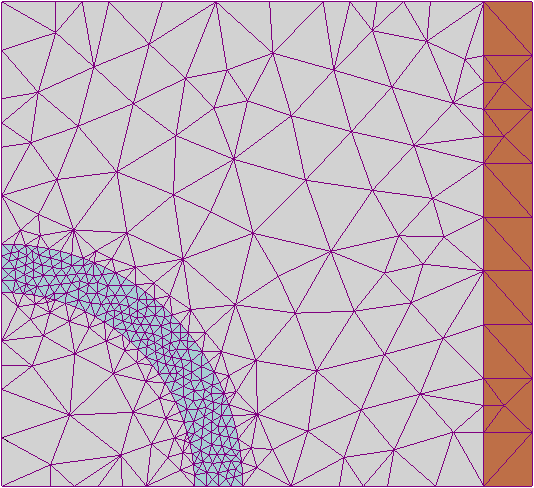
\includegraphics[width=\textwidth]{figures/fem-mesh.png}
  \end{subfigure}
  \begin{subfigure}{.5\textwidth}
    \centering
    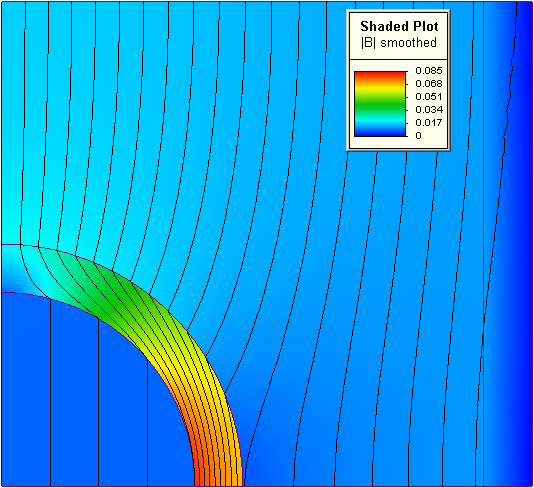
\includegraphics[width=\textwidth]{figures/fem-solution.png}
  \end{subfigure}
  \caption[Παράδειγμα \eng{FEM}]{Αριστερά, διαγραμματικό δίκτυο (\eng{mesh})
    διακριτοποίησης του χώρου προσομοίωσης για επίλυση \eng{FEM} και δεξιά τα αποτελέσματα
    της μεθόδου.}
  \label{fig:fem}
\end{figure}

\paragraph{} Κύριος σκοπός της παρούσας εργασίας ήταν η κατά το δυνατόν ακριβέστερη
καταγραφή της μεταφοράς ορμής/ενέργειας από το τσουνάμι στην ακτογραμμή, για την εκτίμηση
των επιπτώσεων της πρόσκρουσης του τσουνάμι. Αν και ο υπολογισμός της μεταδιδόμενης ορμής
είναι εφικτός με τις παραπάνω μεθόδους, σωματιδιακές μέθοδοι προσομοίωσης προσφέρουν πιο
άμεση πληροφορία σχετικά με αυτή. Σε σύγκριση με τις αριθμητικές μεθόδους, οι σωματιδιακές
μέθοδοι υπερτερούν και σε άλλα σημεία λαμβάνοντας υπόψη πάντα το πρόβλημα (εικόνα
\ref{fig:method-comparison}). Μόνο στην \eng{LBM} από τις δύο σωματιδιακές μεθόδους ο
χώρος της προσομοίωσης διακριτοποιείται, και μάλιστα όχι σε δίκτυο (\eng{mesh}) αλλά
κανονικό πλέγμα (\eng{grid}). Ένα άλλο σημαντικό πλεονέκτημα των σωματιδιακών μεθόδων
είναι η εγγενής διατήρηση ορισμένων ποσοτήτων του ρευστού (μάζα, ορμή, ενέργεια), όπως και
ο αρκετά μικρότερος υπολογιστικός φόρτος για παρόμοιας κλίμακας προσομοιώσεις. Για τους
παραπάνω λόγους, επελέγη σωματιδιακή μέθοδος προσομοίωσης, καθώς τέτοιες μέθοδοι
εν\-δεί\-κνυ\-νται και για την ικανοποίηση οριακών συνθηκών έναντι πολύπλοκης γεωμετρίας
σε ελεύθερες και μη επιφάνειες, χαρακτηριστική επίσης απαίτηση της παρούσας εφαρμογής.

\begin{figure}[h]
  \centering
  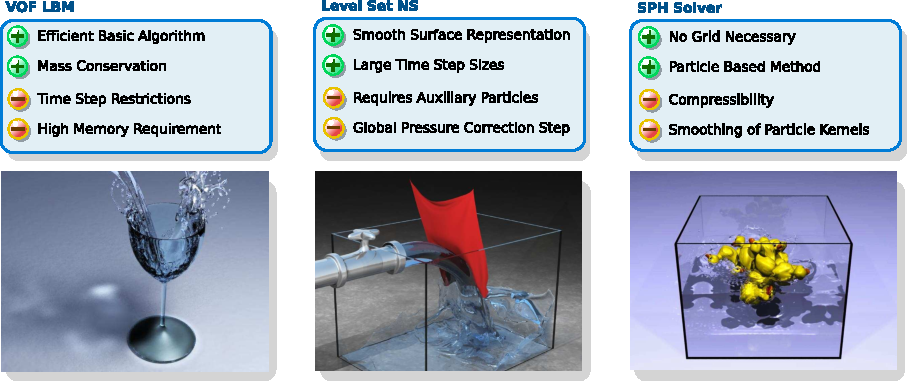
\includegraphics[width=\textwidth]{figures/thuerey-comparison.pdf}
  \caption[Σύγκριση μεθόδων προσομοίωσης] {Σύγκριση τριών μεθόδων προσομοίωσης (από
    \eng{Th{\"u}rey, 2007}) \cite{thuerey2007}}
  \label{fig:method-comparison}
\end{figure}

\subsection{\texorpdfstring{\eng{Lattice Boltzmann Method}}{}}
\paragraph{} Στη βάση της περιγραφής της ρευστοδυναμικής από τις εξισώσεις
\eng{Navier-Stokes} υπάρχει η παραδοχή της συνεχούς φύσης των ρευστών. Υπό αυτήν την
θεώρηση, οι ιδιότητες του ρευστού όπως η πυκνότητα, η πίεση, και η ταχύτητα διατυπώνονται
ως συνεχή πεδία (βαθμωτά ή διανυσματικά), τα οποία μεταβάλλονται στο χώρο και το χρόνο. Σε
αντίθεση με τη μακροσκοπική αυτή θεώρηση έρχεται η μικροσκοπική άποψη των ρευστών, όπου
περιγράφονται σαν σύνολο σωματιδίων, το καθένα από τα οποία έχει συγκεκριμένες μηχανικές
ιδιότητες και συμπεριφορά. Ενδιάμεσα αυτών των δύο βρίσκεται το μεσοσκοπικό επίπεδο, όπου
το ρευστό περιγράφεται ώς συνάρτηση πυκνότητας πιθανότητας $f(\vec{r}, \vec{v}, t)$ της
εύρεσης ενός σωματιδίου στη θέση $\vec{r}$ έχοντας ταχύτητα $\vec{v}$ τη χρονική στιγμή
$t$. H κινητική θεωρία περιγράφει το επίπεδο αυτό μέσω της εξίσωσης \eng{Boltzmann}, στην
οποία βασίζεται και η \eng{LBM} \cite{chen1998}:
\[
\frac{\partial f}{\partial t} +
\frac{\vec{p}}{m} \cdot \nabla f +
\vec{F} \cdot \frac{\partial f}{\partial \vec{p}} =
\left( \frac{\partial f}{\partial t} \right)_{\hspace{-2pt}\text{\eng{coll}}},
\]
όπου $f$ η συνάρτηση κατανομής των σωματιδίων του ρευστού στον εξαδιάστατο χώρο κατάστασης
του συστήματος (θέση $\vec{r}$ και ορμή $\vec{p}$), $m$ η μάζα των σωματιδίων, $\vec{F}$
το πεδίο εξωτερικών δυνάμεων που επιδρούν στα σωματίδια, ενώ το δεξί μέλος ισούται με τη
μεταβολή της $f$ λόγω συγκρούσεων μεταξύ των σωματιδίων. Στην παραπάνω σχέση, το αριστερό
μέλος εκφράζει την ελέυθερη μεταφορά των σωματιδίων, ενώ το δεξί μέλος την αλλαγή στην
κατανομή πιθανότητας που οφείλεται στις συγκρούσεις μεταξύ τους.

\subsubsection{Θεωρητική περιγραφή}
\paragraph{} Κατά την προσομοίωση ρευστών με την \eng{LBM} εκτός του χρόνου
διακριτοποιείται και ο χώρος κατάστασης του συστήματος. Ο τρισδιάστατος χώρος χωρίζεται σε
κυβικά κελιά που σχηματίζουν ένα κανονικό πλέγμα (\eng{grid}), ενώ οι ταχύτητες
κβαντίζονται σε συνιστώσες που οδηγούν από κάθε κελί σε ένα αριθμό γειτονικών κελιών σε
κάποια τάξη συμμετρίας. Τα διάφορα πλέγματα λαμβάνουν την ονομασία τους από τη μορφη
\eng{DXQY}, όπου \eng{X} ο αριθμός των διαστάσεων του χώρου της προσομοίωσης και \eng{Y} ο
αριθμός συνιστωσών ταχύτητας (εικόνα \ref{fig:lb-lattices}). Μετά τη διακριτοποίηση, η
εξίσωση \eng{Boltzmann} μετατρέπεται στην εξίσωση \eng{lattice Boltzmann}:
\[
  f_i(\vec{r} + \vec{e}_i \delta_t, t + \delta_t) =
  f_i(\vec{r},t) - \frac{1}{\tau_f} (f_i - f_i^{\text{\eng{eq}}})
\]
Στη σχέση αυτή, η $f$ είναι πλέον συνάρτηση μάζας πιθανότητας η οποία εκφράζει την
πιθανότητα εύρεσης σωματιδίου στη θέση $\vec{r}$ τη χρονική στιγμή $t$ με ταχύτητα
$\vec{v}$ κατά τη φορά του $\vec{e}_i$, του μοναδιαίου διάνυσματος κατα τη φορά της
$i$-οστής εκ των κβαντισμένων συνιστωσών ταχύτητας, ενώ με $\tau_f$ συμβολίζεται ο
συντελεστής χαλάρωσης προς την κατάσταση ισορροπίας $f_i^{\text{\eng{eq}}}$. Σύμφωνα με τη
σχέση αυτή, το μέρος του ρευστού στο κελί με θέση $\vec{r}$ που έχει ταχύτητα κατά
$\vec{e}_i$ τη χρονική στιγμή $t$ μεταφέρεται στο κελί προς την κατεύθυνση αυτή (στη θέση
$\vec{r} + \vec{e}_i\delta_t$) στην επόμενη χρονική στιγμή $t+\delta_t$, αφού πρώτα σε
κάποιο βαθμό έχει αποκατασταθεί η ισορροπία \eng{equilibrium} του ρευστού. Η ισορροπία
αυτή αντιπροσωπεύει τη χαλάρωση (\eng{relaxation}) του συστήματος μέσω των συγκρούσεων
μεταξύ των σωματιδίων. H σταθερά χαλάρωσης $\tau_f$ καθορίζει τη γραμμική παρεμβολή μεταξύ
της $f_i$ και της $f_i^{\text{\eng{eq}}}$, ρυμίζοντας με αυτόν τον τρόπο έμμεσα το ιξώδες
του ρευστού. Πράγματι η $\tau_f$ είναι ανάλογη του ιξώδους, καθώς όσο αυτή λαμβάνει
μεγαλύτερες τιμές οι $f_i$ περνούν από κελί σε κελί σχεδόν απαράλλαχτες με αποτέλεσμα
ομαλή ροή (\eng{inviscid flow}), ενώ μικρή τιμή της συνεπάγεται σχετικά μεγάλη προσαρμογή
προς την κατάσταση ισορροπίας (μέγιστης εντροπίας) σε κάθε βήμα, οδηγώντας σε ταραχώδη ροή
(\eng{turbulent flow}).

\begin{figure}[]
  \centering
  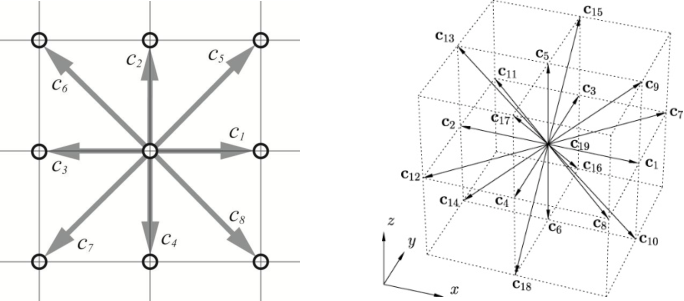
\includegraphics[width=\textwidth]{figures/lb-lattices-2.pdf}
  \caption[Διακριτοποίηση χώρου κατάστασης \eng{LBM}] {Διαφορετικές διακριτοποιήσεις του
    χώρου ταχυτήτων για την μέθοδο \eng{LBM}, αριστερά \eng{D2Q9} και δεξιά \eng{D3Q19}
    (από \eng{Duchateau, 2015} \cite{duchateau2015}). Η ονομασία των διακριτοποιήσεων
    ακολουθεί τον αριθμό των διαστάσεων του χώρου της προσομοίωσης (\eng{D3} για τον
    τρισδιάστατο χώρο) και τον αριθμό των συνιστώσεων στις οποίες κβαντίζεται ο χώρος
    ταχύτητας (\eng{QX} για \eng{X} συνιστώσες)}
  \label{fig:lb-lattices}
\end{figure}

\paragraph{} Κατά τη διάρκεια της προσομοίωσης, οι υπολογισμοί που υπαγορεύονται από την
διακριτοποιημένη εξίσωση \eng{Boltzmann} λαμβάνουν χώρα σε δύο αλληλοδιάδοχα βήματα
συ\-γκρού\-σης (\eng{collision}) και μεταφοράς (\eng{streaming}):
\begin{itemize}
\item[] \makebox[2.5cm]{Σύγκρουση:\hfill}
  $f_i(\vec{r},t+\delta_t) = f_i(\vec{r},t) - \frac{1}{\tau_f} (f_i -
  f_i^{\text{\eng{eq}}})$
\item[] \makebox[2.5cm]{Μεταφορά:\hfill}
  $f_i(\vec{r}+\vec{e}_i\delta_t, t+\delta_t)=f_i(\vec{r},t+\delta_t)$
\end{itemize}
Στο πρώτο από αυτά τα βήματα υπολογίζονται οι νέες $f_i$ μετά το χειρισμό των οριακών
συνθηκών και την αποκατάσταση της ισορροπίας, ενώ στο δεύτερο αυτές μεταφέρονται στα κελιά
προορισμού τους κατά τη φορά της συνιστώσας στην οποία αντιστοιχούν. Ο περισσότερος
υπολογιστικός φόρτος βρίσκεται στο βήμα της σύγκρουσης, όπου υπολογίζονται οι νέες $f_i$
που θα μεταφερθούν στα γειτονικά κελιά στο επόμενο βήμα. Ο υπολογισμός αυτός
αντιπροσωπεύει την κανονικοποίηση και αναδιανομή της πυκνότητας και ορμής του ρευστού,
καθώς για τις $f_i$ ισχύει:
\[
\rho = \sum_if_i \hspace{0.5cm} \text{και} \hspace{0.5cm} \rho\vec{v} = \sum_if_i\vec{e}_i
\]
Εάν ο τελεστής σύγκρουσης παρασταθεί ως $\Omega_i$, τότε η διατήρηση της μάζας και της
ορμής σε κάθε κελί εκφράζεται ως
\[
  \sum_i\Omega_i=0 \hspace{0.5cm} \text{και} \hspace{0.5cm}
  \sum_i\Omega_i\vec{e}_i=\vec{0}
\]
Λαμβάνοντας υπόψη τους παραπάνω περιορισμούς, η κατανομή ισορροπίας
$f_i^{\text{\eng{eq}}}$ υπολογίζεται από τον παρακάτω τύπο \cite{qian1992lattice}:
\[
  f_i^{\text{\eng{eq}}} = \rho w_i \left[
    1
    + 3\vec{e}_i \cdot \vec{v}
    + \frac{9}{2}(\vec{e}_i \cdot \vec{v})^2
    - \frac{3}{2}v^2
  \right]
\]
Τα βάρη $w_i$ είναι συντελεστές κανονικοποιημένοι ώστε να έχουν άθροισμα ίσο με τη μονάδα,
και προκύπτουν ξεχωριστοί για κάθε τάξη πλέγματος διακριτοποίησης, σύμφωνα με τη συνάρτηση
βάρους που χρησιμοποιείται για την προσέγγιση της κατανομής ισορροπίας. Στον πίνακα
\ref{tab:lb-weights} απεικονίζονται για παράδειγμα τα βάρη για κάποιες μορφές πλεγμάτων.
\begin{center}
  \begin{tabular}{ccccc}
    \toprule
    \eng{Lattice & $w_0$ & $w_1$ & $w_2$ & $w_3$} \\
    \midrule
    \eng{D1Q3} & 2/3 & 1/6 & 0 & 0 \\
    \eng{D2Q9} & 4/9 & 1/9 & 1/36 & 0 \\
    \eng{D3Q15} & 2/9 & 1/9 & 0 & 1/72 \\
    \eng{D3Q19} & 1/3 & 1/18 & 1/36 & 0 \\
    \eng{D4Q25} & 1/3 & 1/36 & 0 & 0 \\
    \bottomrule
  \end{tabular}
  \captionof{table}{Τα βάρη για κάθε ομάδα συμμετρικών συνιστωσών της κατανομής ισορροπίας
    $f_i^{\text{\eng{eq}}}$ για διάφορα πλέγματα (από \eng{Qian et al, 1992}
    \cite{qian1992lattice}).}
  \label{tab:lb-weights}
\end{center}

\paragraph{} Ένα από τα κύρια πλεονεκτήματα της \eng{LBM} είναι η ικανότητα εύκολης,
κατανεμημένης διαχείρισης των οριακών συνθηκών, ιδιαίτερα σε όρια που χαρακτηρίζονται από
περίπλοκη ή/και μεταβαλλόμενη γεωμετρία, μέσω απλών χειρισμών στις τιμές των συναρτήσεων
κατανομής. Πολλές τεχνικές έχουν προταθεί, καθεμιά από τις οποίες διαθέτει πλεονεκτήματα
και μειονεκτήματα που αφορούν τα υπολογιστικά της χαρακτηριστικά (πολυπλοκότητα,
τοπικότητα) αλλά και τις ιδιαιτερότητες της εκάστοτε εφαρμογής \cite{chen1998,
  latt2008}. Ως ένα απλό και αντιπροσωπευτικό παράδειγμα μπορεί να αναφερθεί η απλή
τεχνική της αναπήδησης (\eng{bounce-back}), όπου το ρευστό που βρίσκεται σε οριακό κελί
και έχει ταχύτητα προς το όριο, αναπηδά με την ίδια ταχύτητα προς τα πίσω στο επόμενο
χρονικό βήμα, αναστρέφοντας την κάθετη στο όριο συνιστώσα της ταχύτητας. Η παράλληλη
συνιστώσα μπορεί είτε να μηδενιστεί (\eng{no-slip}) είτε να αφεθεί ως έχει
(\eng{free-slip}) για το χρονικό αυτό βήμα, αναλόγως της εφαρμογής. Με τον τρόπο αυτό
εξασφαλίζεται μηδενική ροή από και προς το όριο, ανεξάρτητα της γεωμετρικής του
πολυπλοκότητας.

\subsubsection{Εφαρμογές}
\paragraph{} Η μέθοδος διαθέτει αρκετά πλεονεκτήματα τα οποία την καθιστούν ελκυστική σε
ορισμένες εφαρμογές. Λόγω της τοπικότητας και κανονικότητας της επεξεργασίας και κίνησης
των δεδομένων ταιριάζει ιδιαίτερα σε \eng{SIMD} αρχιτεκτονικές παράλληλης επεξεργασίας, οι
οποίες τα τελευταία χρόνια παρουσιάζουν τεράστια ανάπτυξη (όπως \eng{GPGPUs}). Πράγματι,
έχει δειχθεί \cite{Bailey2009550} οτι η μέθοδος εκτελείται ταχύτερα σε \eng{GPUs} σε σχέση
με \eng{FPGAs} και γενικού σκοπού επεξεργαστές. Στην ίδια μελέτη αυτό επιβεβαιώνεται από
μια βελτιωμένη υλοποίηση της \eng{LBM} σε \eng{GPUs}, χρησιμοποιώντας το πλέγμα
\eng{D3Q19}, η οποία ήταν πάνω από 28 φορές ταχύτερη από αντίστοιχη έκδοση για τετραπύρηνο
επεξεργαστή επάνω στην πλατφόρμα παραλληλης επεξεργασίας \eng{OpenMP}. Η εύκολη και
αποδοτική παραλληλοποίηση της μεθόδου έχει οδηγήσει στη χρήση της σε ολοένα και πιο
καινοτόμες εφαρμογές. Επί παραδείγματι, πρόσφατα ο αλγόριθμος χρησιμοποιήθηκε ως μέθοδος
επίλυσης της εξίσωσης \eng{level set} για την τμηματοποίηση (\eng{segmentation}) εικόνας
\cite{balla-arabe2011}, αλλά και για προσομοίωση αλληλεπίδρασης ρευστού με στερεά όρια
(\eng{Fluid-Structure Interaction -- FSI}) \cite{nita2015}. Στην τελευταία αυτή εργασία η
μέθοδος επεκτάθηκε προκειμένου να λάβει υπόψη την κινούμενη γεωμετρία των αιμοφόρων
αγγείων καθώς αυτά αναπαρίσταντο από τρισδιάστατο μοντέλο. Πίσω στο πεδίο της
ρευστομηχανικής, η μέθοδος συνεχίζει να χρησιμοποιείται εκτενώς σε πληθώρα προβλημάτων,
μεταξύ των οποίων και αυτά που άπτονται της παρούσας εργασίας. Σημαντική δουλειά έχει
γίνει στη χρήση της μεθόδου για προσομοίωση φαινομένων που άπτονται της παρούσας εργασίας
τόσο σε θεωρητικό όσο και τεχνικό επίπεδο. Σε θεωρητικό επίπεδο, οι εξισώσεις ρηχού νερού
(\eng{Shallow Water Equations}), οι οποίες είναι απλοποιημένες μορφές της εξίσωσης
\eng{Navier-Stokes} για περιπτώσεις όπου το οριζόντιο χαρακτηριστικό μήκος ροής είναι πολύ
μεγαλύτερο από το βάθος του νερού έχουν μοντελοποιηθεί σύμφωνα με την \eng{LBM},
λαμβάνοντας υπόψη παράγοντες όπως η κλίση και τριβή του πυθμένα με εξαιρετική συμφωνία να
παρατηρείται μεταξύ προσομοιώσεων και αναλυτικών λύσεων \cite{Zhou20023527,
  Zhou2004lattice}. Σε άλλη μελέτη, η προσομοίωση της διάδοσης τσουνάμι βάσει των μη
γραμμικών εξισώσεων ρηχού νερού με χρήση της \eng{LBM} σε \eng{GPU} αποδείχθηκε αξιόπιστη,
καθώς τα αποτελέσματά της ήταν σύμφωνα με τις λύσεις σε πρότυπα προβλήματα
\cite{Janssen2012efficient}. Αντίστοιχα για την πρόσκρουση και τις επιπτώσεις ενός
τσουνάμι σε επίπεδο ακτογραμμής η \eng{LBM} έχει προταθεί για τη χρησιμότητά της στην
εκτίμηση της ταχύτητας και επιπέδων ροής αλλά και των δυνάμεων που ασκεί το κύμα στην
ακτογραμμή \cite{Krafczyk2007}.

\paragraph{} Συνολικά, η \eng{LBM} διαθέτει μεγάλο θεωρητικό υπόβαθρο και αποτελεί
αντικείμενο ενεργούς έρευνας για τη διεύρυνση και βελτίωση των εφαρμογών της προς κάθε
κατεύθυνση. Η μέθοδος διακρίνεται για την ευκολία με την οποία χειρίζεται ροές πολλαπλών
φάσεων και συστατικών (\eng{multiphase -- multicomponent}) που πιθανόν αλληλεπιδρούν με
ιδιαίτερο τρόπο αλλά και περίπλοκη γεωμετρία ορίων (όπως πορώδη μέσα). Η εγγενής
παραλληλία σε συνδυασμό με την τοπικότητα του αλγορίθμου την καθιστούν κατάλληλη σε
εφαρμογές μεγάλου όγκου δεδομένων, καθώς λόγω αυτών χρησιμοποιείται με εξαιρετικά
αποτελέσματα σε παράλληλες αρχιτεκτονικές \eng{SIMD (GPUs)}. Ωστόσο αποτελεί μια νέα
σχετικά μέθοδο, η οποία αν και πολλά υποσχόμενη χρησιμοποιείται ακόμη ως επί το πλείστον
σε ερευνητικές και αρκετά λιγότερο σε πρακτικές εφαρμογές.

\subsection{\texorpdfstring{\eng{Smoothed Particle Hydrodynamics}}{}}
\paragraph{} Η \eng{SPH} είναι μια Λαγκρανζιανή μέθοδος προσομοίωσης ρευστών που εισήχθη
τη δεκαετία του 1970 για προσομοίωση αστροφυσικών φαινομένων \cite{gingold1977375,
  lucy19771013} και έκτοτε έχει βρει ευρύτατη εφαρμογή σε πολλά επιστημονικά πεδία, όπως η
βαλλιστική, αεροδυναμική, ναυπηγική και γραφικά \cite{monaghan20051703}. Οι Λαγκρανζιανές
μέθοδοι διαφέρουν από τις Οϊλεριανές στην επιλογή του σημείου αναφοράς κατά την περιγραφή
του ρευστού. Στις Λαγκρανζιανές μεθόδους, ως σημείο αναφοράς λαμβάνεται ένα τμήμα
(\eng{fluid parcel}) του ρευστού, ακολουθώντας τη ροή του, ενώ στις Οϊλεριανές η περιγραφή
γίνεται με πεδία μεγεθών ορισμένα με σημείο αναφοράς τις συντεταγμένες του τρισδιάστατου
χώρου. Θεμέλιο της μεθόδου αποτελεί η αντικατάσταση του ρευστού από ένα σύνολο σωματιδίων,
τα οποία φέρουν ιδιότητες του ρευστού και αποτελούν σημεία παρεμβολής για τον υπολογισμό
αυτών σε άλλα σημεία του χώρου, λόγω του οποίου διαθέτει αρκετά πλεονεκτήματα:
\begin{itemize}
\item Εγγενής διατήρηση πολλών μεγεθών στο σύστημα λόγω της σωματιδιακής του φύσης, όπως
  μάζα, ορμή και ενέργεια.
\item Ακριβής, ισότροπος και αμετάβλητος σε κάθε αδρανειακό σύστημα αναφοράς
  (\eng{Galilean invariant}) χειρισμός της καθαρής μεταφοράς (\eng{pure advection})
\item Δυνατότητα προσαρμογής της αναλυτικότητας (\eng{resolution}) και κατά συνέπεια του
  υπολογιστικού φόρτου δυναμικά συναρτήσει της θέσης, χρόνου ή άλλων παραγόντων.
\item Εύκολος χειρισμός ορίων και ειδικών αλληλεπιδράσεων σε εφαρμογές πολλαπλών φάσεων
  και συστατικών, μέσω των σωματιδιακών αλληλεπιδράσεων.
\end{itemize}

\subsubsection{Θεωρητική θεμελίωση}
\paragraph{} Η \eng{SPH} βασίζεται στη διακριτοποίηση του ρευστού, με το χωρισμό του σε
σωματίδια που φέρουν τις ιδιότητές του, μέσω της οποίας πραγματοποιείται ουσιαστικά η
μετάβαση από την Οϊλεριανή θεώρηση στη Λαγκρανζιανή. Για τη δειγματοληψία μιας συνάρτησης
$f$ που περιγράφεται συναρτήσει της θέσης $\vec{r}$ στο χώρο $V$, ισχύει η ταυτότητα
\begin{equation}
  f(\vec{r}) = \int_Vf(\vec{x}) \delta(\vec{r} - \vec{x}) d\vec{x},
\end{equation}
όπου, $\delta(\vec{r})$ η συνάρτηση δέλτα του \eng{Dirac} και $\vec{x} \in V$. Η συνάρτηση
δέλτα μπορεί να θεωρηθεί η οριακή περίπτωση ενός πυρήνα εξομάλυνσης $W(\vec{r}, h)$ με τις
εξής ιδιότητες
\begin{equation}
  \label{eq:kernel-properties}
  \lim_{h\to0}W(\vec{r}, h) = \delta(\vec{r})\ \ \
  \text{και}\ \ \
  \int_VW(\vec{r}, h) d\vec{x} = 1
\end{equation}
Τότε, για μικρές τιμές του $h$ ισχύει
\begin{equation}
  \label{eq:c-approx}
  f(\vec{r}) \approx \int_V f(\vec{x}) W(\vec{r}-\vec{x}, h) d\vec{x}
\end{equation}
Αφού διακριτοποιήσουμε το πεδίο $f$ σε σωματίδια πυκνότητας $\rho_i$ και μάζας $m_i$
μπορούμε να πολλαπλασιάσουμε και να διαιρέσουμε με $\rho$ το δεξί μέλος της παραπάνω
σχέσης, το οποίο μετατρέπεται πλέον σε διακριτό άθροισμα.  Παρατηρώντας ότι
$\rho*d\vec{x} = m$, καταλήγουμε στην ακόλουθη σχέση που αποτελεί τη βάση προσέγγισης
οποιουδήποτε μεγέθους $A$ σύμφωνα με την \eng{SPH}
\begin{equation}
  \label{eq:d-approx}
  A(\vec{r}) \approx \sum_i \frac{m_i}{\rho_i} A(\vec{r}_i) W(\vec{r}-\vec{x}_i, h)
\end{equation}
Σύμφωνα με αυτή, η τιμή της $A$ σε μια θέση του χώρου $\vec{r}$ μπορεί να υπολογιστεί
προσεγγιστικά απο το σταθμισμένο άθροισμα των τιμών της στα γειτονικά σωματίδια $i$.  Η
συνεισφορά κάθε σωματιδίου καθορίζεται τόσο από το λόγο της μάζας του προς την τοπική
πυκνότητα $m_i/\rho_i$, όσο και από την απόστασή του από το σημείο υπολογισμού της $A$
μέσω του πυρήνα $W(\vec{r}-\vec{x}_i, h)$.

\subsubsection{Διανυσματικοί τελεστές σε διακριτοποιημένα πεδία}
\label{sssec:vector-calc}
\paragraph{} Δεδομένου ότι $\nabla \equiv \partial/\partial\vec{r}$,
από τη σχέση \ref{eq:d-approx} για τη βάθμωση του μεγέθους $A$ προκύπτει
\begin{equation}
  \label{eq:d-grad}
  \nabla A(\vec{r}) \approx \sum_i \frac{m_i}{\rho_i} A(\vec{r}_i) \nabla W(\vec{r} - \vec{x}_i, h)
\end{equation}
Αντίστοιχα, για την απόκλιση και το στροβιλισμό του διανυσματικού μέγεθους $\vec{A}$
\begin{equation}
  \label{eq:d-div}
  \nabla \cdot \vec{A}(\vec{r}) \approx \sum_i \frac{m_i}{\rho_i} \vec{A}(\vec{r}_i)
  \cdot \nabla W(\vec{r} - \vec{x}_i, h)
\end{equation}
\begin{equation}
  \label{eq:d-curl}
  \nabla \times \vec{A}(\vec{r}) \approx \sum_i \frac{m_i}{\rho_i} \vec{A}(\vec{r}_i)
  \times \nabla W(\vec{r} - \vec{x}_i, h)
\end{equation}
Αξίζει να σημειωθεί η εξάρτηση της προσέγγισης αποκλειστικά από τις τιμές της συνάρτησης
$A(\vec{r}_i)$/$\vec{A}(\vec{r}_i)$ και της βάθμωσης του πυρήνα εξομάλυνσης $\nabla W$,
χαρακτηριστικό ιδιαίτερα χρήσιμο υπολογιστικά, καθώς η τελευταία μπορεί να προϋπολογιστεί.

\paragraph{} Οι παραπάνω σχέσεις μπορούν να τροποποιηθούν για την ικανοποίηση ειδικών
συνθηκών της εκάστοτε εφαρμογής. Στην παρούσα περίπτωση απαιτείται η διατήρηση της ορμής
στο ρευστό, η οποία μεταφράζεται στην εξασφάλιση αντισυμμετρικών δυνάμεων (δράσης -
αντίδρασης) μεταξύ των σωματιδίων του ρευστού. Σύμφωνα με την εξίσωση \eng{Navier-Stokes}
(σχέση \ref{eq:navier-stokes}), οι εσωτερικές δυνάμεις του ρευστού οφείλονται στη βάθμωση
του πεδίου πίεσης και το γινόμενο του δυναμικού ιξώδους με τη λαπλασιανή του πεδίου
ταχύτητας. Μπορούμε να καταλήξουμε σε διαφορετικό εκτιμητή για τη βάθμωση της πίεσης
ξεκινώντας από την ταυτότητα
\begin{equation*}
  \label{eq:grad-identity}
  \nabla \left( \frac{P}{\rho} \right) =
  \frac{\nabla P}{\rho}-
  \frac{P}{\rho^2} \nabla \rho
  \hspace{10pt} \Leftrightarrow \hspace{10pt}
  \nabla P = \rho \left[ \frac{P}{\rho^2} \nabla \rho + \nabla \left( \frac{P}{\rho}
    \right) \right]
\end{equation*}
Αντικαθιστώντας στο δεξί μέλος τις βαθμώσεις με τους εκτιμητές τους κατά \eng{SPH}
\begin{align}
  \label{eq:grad-est}
  \nabla P &\approx \rho \left[ \frac{P}{\rho^2} \sum_i \frac{m_i}{\rho_i} \rho \nabla
             W(\vec{r}-\vec{r}_i, h)
             +
             \sum_i \frac{m_i}{\rho_i} \frac{P_i}{\rho_i} \nabla W(\vec{r}-\vec{r}_i, h)
             \right] \nonumber \\
           &\approx\rho \sum_i m_i \left(\frac{P}{\rho^2} + \frac{P_i}{\rho_i} \right)
             \nabla W(\vec{r}-\vec{r}_i, h)
\end{align}
προκύπτει η σχέση που χρησιμοποιείται ευρύτατα για την εκτίμηση της βάθμωσης της πίεσης
και ικανοποιεί παράλληλα τη συνθήκη αντισυμμετρικότητας για τη διατήρηση της ορμής και
στροφορμής. Παρόμοια, για τη λαπλασιανή του πεδίου ταχύτητας χρησιμοποιείται συνήθως η
προσέγγιση
\begin{equation}
  \label{eq:lapl-est}
  \nabla^2\vec{v} \approx \sum_i \frac{m_i}{\rho_i} (\vec{v}_i - \vec{v}) \nabla^2
  W(\vec{r}-\vec{r}_i, h)
\end{equation}
η οποία διαθέτει την επιθυμητή για την προσομοίωση των δυνάμεων ιξώδους ιδιότητα του
μηδενισμού σε κατάσταση ομοιόμορφης μεταφορικής κίνησης του ρευστού (ίση ταχύτητα στο
εύρος του πυρήνα εξομάλυνσης).

\subsubsection{Καταστατική εξίσωση}
\paragraph{} Για τον υπολογισμό της βάθμωσης της πίεσης είναι απαραίτητος ο υπολογισμός
των τιμών της στα σημεία δειγματοληψίας (σωματίδια). Αυτός γίνεται με τη βοήθεια μιας
καταστατικής εξίσωσης, η οποία συσχετίζει την πυκνότητα με την πίεση του ρευστού. Επομένως
για να εκτιμηθεί η πίεση σε κάποιο σημείο πρέπει πρώτα να εκτιμηθεί η πυκνότητα στο σημείο
αυτό από τη σχέση \ref{eq:d-approx}:
\begin{equation}
  \label{eq:dens-est}
  \rho(\vec{r}) \approx \sum_i m_i W(\vec{r}-\vec{x}_i, h)
\end{equation}
Οι δύο ευρύτερα χρησιμοποιούμενες καταστατικές εξισώσεις είναι αυτή των ιδανικών αερίων
\cite{muller2003particle, desbrun1996smoothed}
\begin{equation}
  \label{eq:ideal-state}
  P = k(\rho - \rho_0),
\end{equation}
που συσχετίζει την πίεση με την απόκλιση από την πυκνότητα αναφοράς $\rho_0$ με μια
σταθερά αναλογίας $k$, καθώς και η εξίσωση \eng{Tait} \cite{becker2007weakly,
  monaghan20051703}
\begin{equation}
  \label{eq:tait-state}
  P = B \left( \left( \frac{\rho}{\rho_0} \right)^\gamma - 1 \right),
\end{equation}
όπου $\gamma=7$ αδιάστατη σταθερά και $B$ σταθερά αναλογίας που ρυθμίζει την ανοχή στις
διακυμάνσεις της πυκνότητας. Η τιμή της $B$ καθορίζεται βάσει της αναλογίας
\begin{equation}
  \label{eq:compressibility-scale}
  \frac{|\Delta\rho|}{\rho_0} \sim \frac{\|\vec{v}_f\|^2}{c_s^2},
\end{equation}
όπου $\Delta\rho = \rho - \rho_0$, $\vec{v}_f$ η ταχύτητα της ροής και $c_s$ η ταχύτητα
του ήχου στο ρευστό. Εάν θέσουμε $\eta = |\Delta\rho|/\rho_0$, τότε ισοδύναμα ισχύει
$c_s \sim \vec{v}_f / \sqrt{\eta}$.  Μπορεί να τεθεί άνω όριο για το $\eta$ (λ.χ.
$\eta = 0.01$ για διακυμάνσεις πυκνότητας της τάξης του $1\%$), το οποίο επιβάλλεται στην
προσομοίωση θέτοντας $B = \rho_0 c_s^2 / \gamma$.  Ωστόσο, για λόγους ευστάθειας, η χρήση
της εξίσωσης \eng{Tait} απαιτεί πολύ μικρό χρονικό βήμα, λόγω της παρουσίας του $c_s^2$
στο συντελεστή αναλογίας $B$.

\subsubsection{Πυρήνες εξομάλυνσης}
\paragraph{} Από τα παραπάνω γίνεται σαφές οτι η επιλογή του πυρήνα εξομάλυνσης είναι
σημαντική, καθώς από αυτήν εξαρτάται άμεσα η ακρίβεια των προσεγγίσεων στο
διακριτοποιημένο ρευστό. Ο πυρήνας εξομάλυνσης θα πρέπει να ικανοποιεί τις σχέσεις
\ref{eq:kernel-properties}, να είναι συνεχής και παραγωγίσιμος (για τον υπολογισμό των
προσεγγίσεων διαφορικών τελεστών) καθώς και σφαιρικά συμμετρικός, ώστε οι τιμές του να
εξαρτώνται αποκλειστικά από την απόσταση από το κέντρο του $r = \|\vec{r}-\vec{r}_i\|$ και
την ακτίνα εξομάλυνσης $h$. Συνήθως χρησιμοποιούνται διαφορετικοί πυρήνες για κάθε
προσεγγιζόμενο μέγεθος, αναλόγως των ειδικών συνθηκών που απαιτούνται για την προσομοίωση
της συμπεριφοράς που αυτό προκαλεί \cite{muller2003particle}

\begin{figure}[h]
  \centering
  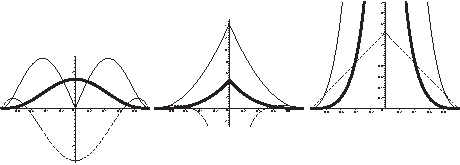
\includegraphics[width=\textwidth]{figures/smoothing-kernels.pdf}
  \caption[Πυρήνες εξομάλυνσης] {Οι τρεις πυρήνες εξομάλυνσης $W_{\text{\eng{poly6}}}$
    $W_{\text{\eng{spiky}}}$ και $W_{\text{\eng{viscosity}}}$ (από δεξιά προς τα
    αριστερά). Με τονισμένη γραμμή απεικονίζεται ο πυρήνας, με λεπτή η βάθμωσή του (στην
    κατεύθυνση προς την αρχή των αξόνων) και με διακεκομένη η λαπλασιανή του, για ακτίνα
    εξομάλυνσης $h=1$.  (από \eng{M{\"u}ller et al, 2003}) \cite{muller2003particle}}
  \label{fig:smoothing-kernels}
\end{figure}

\paragraph{} Στο σχήμα \ref{fig:smoothing-kernels} φαίνονται οι τρεις πυρήνες
$W_{\text{\eng{poly6}}}$, $W_{\text{\eng{spiky}}}$ και $W_{\text{\eng{viscosity}}}$ που
χρησιμοποιούνται πρακτικά για τον υπολογισμό της πυκνότητας, της βάθμωσης της πίεσης και
της λαπλασιανής του πεδίου ταχύτητας αντίστοιχα. Είναι σημαντικό για την ευστάθεια της
προσομοίωσης, αλλά και λογικό από φυσικής εποπτείας οι πυρήνες και οι παράγωγοι τους να
τείνουν στο μηδέν στα όρια της ακτίνας εξομάλυνσης. Για τον υπολογισμό της πυκνότητας
χρησιμοποιείται ο πυρήνας
\begin{equation}
  \label{eq:poly6}
  W_{\text{\eng{poly6}}}(r, h) = \frac{315}{64 \pi h^9}
  \begin{cases}
    (h^2 - r^2)^3 & 0 \leq r \leq h\\
    0 & \text{διαφορετικά}
  \end{cases}
\end{equation}
ο οποίος είναι τυπικός κωδωνοειδής πληρώντας τα χαρακτηριστικά που αναφέρθηκαν
προηγουμένως. Παρ' όλ' αυτά δε χρησιμοποιείται για την προσέγγιση της βάθμωσης της πίεσης,
καθότι η μηδενική παράγωγος στο κέντρο οδηγεί σε συσσωμάτωση (\eng{clustering}) των
σωματιδίων λόγω απουσίας απωστικών δυνάμεων μεταξύ τους. Για το λόγο αυτό, έχει προταθεί
\cite{desbrun1996smoothed} ο πυρήνας
\begin{equation}
  \label{eq:spiky}
  W_{\text{\eng{spiky}}}(r, h) = \frac{15}{\pi h^6}
  \begin{cases}
    (h - r)^3 & 0 \leq r \leq h\\
    0 & \text{διαφορετικά}
  \end{cases}
\end{equation}
\begin{equation}
  \label{eq:spiky-gradient}
  \nabla W_{\text{\eng{spiky}}}(r, h) = \frac{-45}{\pi h^6} (h-r)^2
\end{equation}
για τον υπολογισμό των δυνάμεων οφειλομένων στη βάθμωση της πίεσης. Ωστόσο οι δυνάμεις
ιξώδους είναι ανάλογες της λαπλασιανής του πυρήνα, με αποτέλεσμα οι παραπάνω πυρήνες να
είναι ακατάλληλοι για την προσέγγισή τους. Δεδομένου οτι οι δυνάμεις αυτές οφείλονται στην
εσωτερική τριβή του ρευστού, έχουν πάντα αποσβεστικά αποτελέσματα αμβλύνοντας τις τοπικές
διαφορές στην ταχύτητά του. Αντίθετα, οι λαπλασιανές των παραπάνω πυρήνων αλλάζουν αλλάζει
πρόσημο παίρνοντας αρνητικές τιμές. Έτσι υιοθετείται ο πυρήνας
\begin{equation}
  \label{eq:viscosity}
  W_{\text{\eng{viscosity}}}(r, h) = \frac{15}{2 \pi h^3}
  \begin{cases}
    - \frac{r^3}{2h^3} + \frac{r^2}{h^2} + \frac{h}{2r} - 1 & 0 \leq r \leq h\\
    0 & \text{διαφορετικά},
  \end{cases}\\
\end{equation}
\begin{equation}
  \label{eq:viscosity-laplacian}
  \nabla^2 W_{\text{\eng{viscosity}}}(r, h) = \frac{45}{\pi h^6} (h-r)
\end{equation}
ο οποίος έχει παντού θετική λαπλασιανή, της οποίας η γραμμικότητα συμβάλλει περαιτέρω στην
ευστάθεια της προσομοίωσης.

\subsubsection{Ολοκλήρωση και χρονικό βήμα}
\label{sssec:integration}
\paragraph{} Εκτός της επιλογής του πυρήνα, καθοριστική για την ακρίβεια και ευστάθεια της
προσομοίωσης είναι η επιλογη του χρονικού βήματος και της μεθόδου ολοκλήρωσης στο
χρόνο. Το χρονικό βήμα υπολογίζεται συνήθως με βάση το κριτήριο \eng{CFL
  (Courant-Friedrichs-Lewy)} το οποίο στην απλούστερη μορφή του δίνεται από τη σχέση
\begin{equation}
  \label{eq:cfl}
  \delta t_{\text{\eng{CFL}}} = C \frac {\delta x}{v},
\end{equation}
όπου $C$ ο αδιάστατος αριθμός \eng{Courant} (συνήθως $0 < C \leq 1$), $\delta x$ είναι
κάποιο χαρακτηριστικό μήκος και $v$ μια σχετική με αυτό χαρακτηριστική ταχύτητα. Στην
περίπτωση της \eng{SPH} μπορεί να χρησιμοποιηθεί η ακτίνα εξομάλυνσης $h$ ή η ακτίνα των
σωματιδίων σαν $\delta x$, ενώ για την $v$ είτε η ταχύτητα του ήχου στο ρευστο, είτε η
ταχύτητα των σωματιδίων για τη μέγιστη ανεκτή μεταβολή πυκνότητας κατά τη διάρκεια ενός
χρονικού βήματος, είτε η μέγιστη ταχύτητα των σωματιδίων (αν μπορεί αυτή εκ των προτέρων
να εκτιμηθεί με αξιοπιστία και δεν οδηγεί σε μη αποδεκτές μεταβολές πυκνότητας). Μεταβλητό
χρονικό βήμα μπορεί να χρησιμοποιηθεί υπό προϋποθέσεις εξαρτώμενες και από την μέθοδο
ολοκλήρωσης, με την προσαρμογή να λαμβάνει χώρα σε κάθε βήμα της προσομοίωση με βάση το
κριτήριο \eng{CFL} \cite{gomez2010state}. Χρησιμοποιώντας μία μέθοδο ολοκλήρωσης
τουλάχιστον δεύτερης τάξης, το μεταβλητό χρονικό βήμα μπορεί να υπολογιστεί ως εξής:
\begin{align*}
  \Delta t &= C \cdot min(\Delta t_f, \Delta t_{cu})\text{, όπου} \\
  \Delta t_f &= \min_i(\sqrt{h/|f_i|}) \\
  \Delta t_{cu} &= \min_i \frac{h} {c_s + \max_j\left| \frac {h\vec{u}_{ij}\vec{x}_{ij}} {r^2_{ij}} \right|}
\end{align*}
Το χρονικό βήμα που τελικά υιοθετείται είναι το ελάχιστο μεταξύ του χρονικού βήματος
$\Delta t_f$ που υπαγορεύεται από τη μέγιστη επιτάχυνση (δύναμη ανα μονάδα μάζας
συμβολίζεται με $f_i$) που ασκείται σε σωματίδιο και του $\Delta t_{cu}$ που επιτρέπει η
μέγιστη σχετική ταχύτητα μεταξύ σωματιδίων σε συνδυασμό με την ταχύτητα του ήχου, αμφότερα
ως προς την ακτίνα εξομάλυνσης $h$.

\paragraph{} Για την αριθμητική ολοκλήρωση στο χρόνο χρησιμοποιούνται πολλές μέθοδοι,
μεταξύ των οποίων η \eng{predictor-corrector} και η \eng{Runge-Kutta-Fehlberg}. Ίσως η
ευρύτερα διαδεδομένη είναι η οικογένεια των \eng{St{\"o}rmer-Verlet} και \eng{Leapfrog},
οι οποίες είναι μέθοδοι δεύτερης τάξης με χαμηλές υπολογιστικές απαιτήσεις και καλή
αριθμητική ευστάθεια. Η μέθοδος \eng{Leapfrog} οφείλει το όνομά της στον αλληλοδιάδοχο
υπολογισμό της θέσης και της ταχύτας ανα μισό χρονικό βήμα
\begin{align}
  \begin{split}
    \label{eq:leapfrog}
    \vec{r}_{i+1} &= \vec{r}_i + \vec{v}_{i-1/2} \delta t \\
    \vec{v}_{i+1/2} &= \vec{v}_{i-1/2} + \vec{a}_i \delta t
  \end{split}
\end{align}
ή ισοδύναμα, σε ακέραια χρονικά βήματα
\begin{align}
  \begin{split}
    \label{eq:leapfrog}
    \vec{r}_{i+1} &= \vec{r}_i + \left( \vec{v}_i + \vec{a}_i \frac{\delta t}{2} \right) \delta t \\
    \vec{v}_{i+1} &= \vec{v}_i + \frac{\vec{a}_i + \vec{a}_{i+1}}{2} \delta t
  \end{split}
\end{align}
Λόγω της εξάρτησης των δυνάμεων (λ.χ. ιξώδους) και από την ταχύτητα στην \eng{SPH} μπορούν
να χρησιμοποιηθούν διάφορες τεχνικές εκτίμησης για τιμές στο μέλλον, όπως την επιτάχυνση
$\vec{a}_{i+1}$
\cite{rawiraswattana2012dynamics}.  Αυτές προσφέρουν παράλληλα τη δυνατότητα χρήσης
μεταβλητού χρονικού βήματος \cite{springel2001gadget}, η οποία δεν υπάρχει στην απλή
\eng{Leapfrog} μέθοδο, λόγω της εγγενούς συμμετρίας της \cite{skeel1993variable}.

%%% Local Variables:
%%% mode: latex
%%% TeX-master: "report"
%%% End:
